\documentclass[12pt]{article}
\usepackage{charter} % font
\usepackage[margin=1in]{geometry} % margin
\usepackage{hyperref} % hyperlinks
\usepackage{enumitem} % Enumeration
\usepackage{graphicx} % images
\usepackage{float} % image placement
\graphicspath{ {graphs/} } 

%%%%%%%%%%%%%%%%%%%%%%%%%%%%%%%%%%%%%%%%%%%%%%%%%%%%%%%%%%%%%%%%%%%%%%%%%%%%%%%%

\title{%
	\textbf{Assignment 3 \\ 
	Sorting: Putting your affairs in order \\
	\large WRITEUP} }

	\author{Zack Traczyk \\ CSE13S - Spring 2021}
	\date{Due: April 25\textsuperscript{th} at 11:59 pm}

%%%%%%%%%%%%%%%%%%%%%%%%%%%%%%%%%%%%%%%%%%%%%%%%%%%%%%%%%%%%%%%%%%%%%%%%%%%%%%%%

	\begin{document}

	\maketitle

	\section{Time Complexity}

	In this assignment, four sorting algorithms were implemented:
	Bubble Sort, Shell Sort, Quicksort with a stack, and Quicksort with a queue.
	Each algorithm has a different balance of memory usage, comparisons, and swamps resulting in different runtime and Big-$O$ analyses.
	Since the length of the array will be discussed often, this value will be referred to as $n$.
	All of the algorithms were executed using the default random seed 13371453.

	\pagebreak

%%%%%%%%%%%%%%%%%%%%%%%%%%%%%%%%%%%%%%%%%%%%%%%%%%%%%%%%%%%%%%%%%%%%%%%%%%%%%%%%

	\subsection{Bubble Sort}

	Bubble Sort is relatively naive sort, simply switching bordering values until the array is sorted.
	Unsurprisingly, this approach is not efficient for larger arrays.
	Bubble Sort had the worst time complexity out of all the sorts implemented.
	Figure \ref{bubble} displays the relationship between the amount of comparisons the algorithm performs and $n$.
	The algorithm uses two loops:
	an outer while loop that goes until the array is sorted,
	then a for loop to compare each bordering item that is unsorted.
	This computation results in a time complexity of $O(n^2)$, validating the figure \ref{bubble}'s quadratic curve.
	is fairly accurate to the actual algorithm's performance.

	A reversed array requires the most amount of comparisons in bubble sort.
	This is because Bubble Sort operates by moving the largest unsorted element to the top every loop.
	Therefore, if the largest items are being sorted first, they will take the most comparisons to get back to the top.

	The corresponding constant for Bubble Sort's $O(n^2)$ complexity is relatively small.
	The algorithm does not create any data structures and has no need to access any memory besides the given array.
	Furthermore, each iteration only occurs once, and decreases each pass since the items at the end are sorted.
	This means the actual complexity is closer to $n^2 - n$ which can make a difference in small arrays (i.e. less than 50 items). 


	\begin{figure}[H]
		\caption{Bubble Sort}\label{bubble}
		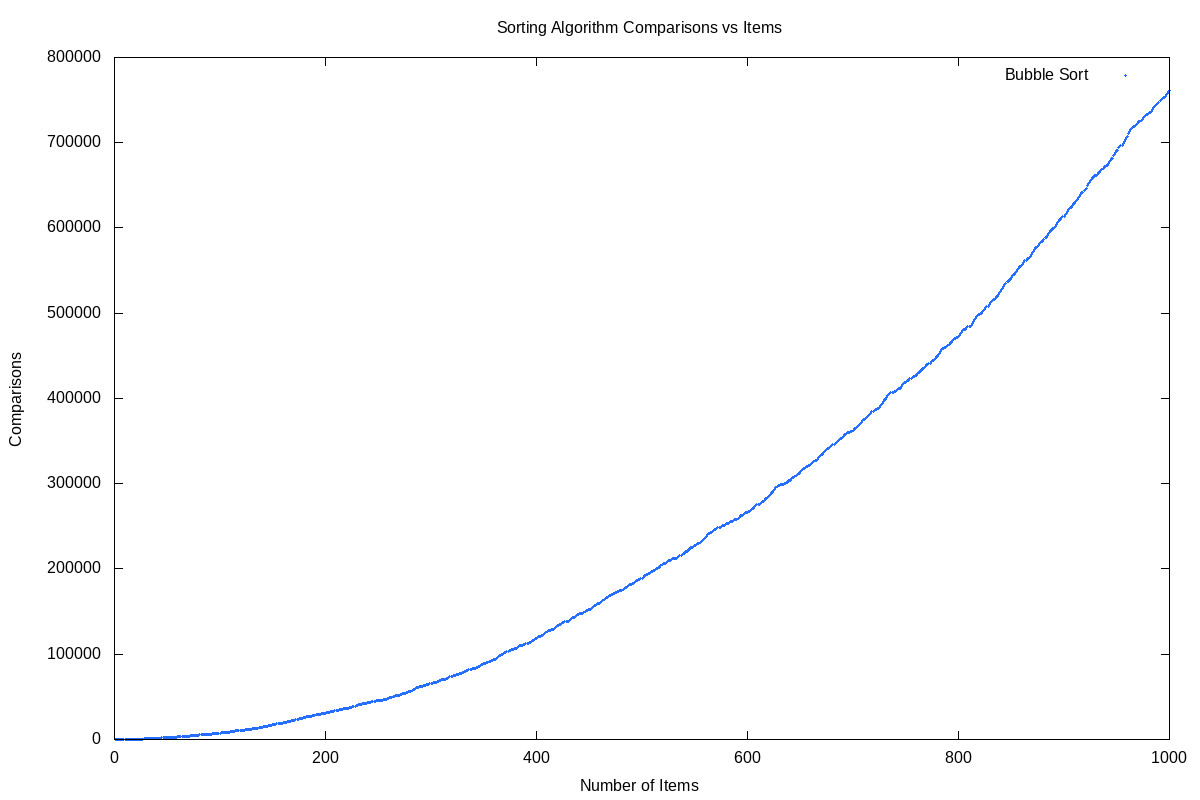
\includegraphics[width=6in]{bubble}
		\centering
	\end{figure}

%%%%%%%%%%%%%%%%%%%%%%%%%%%%%%%%%%%%%%%%%%%%%%%%%%%%%%%%%%%%%%%%%%%%%%%%%%%%%%%%

	\subsection{Shell Sort}

	Shell sort preformed much better than Bubble Sort.
	Just by looking at figure \ref{shell} the curve is obviously less slopped than figure \ref{bubble}.
	Shell Sort's worst case scenario is $O(n^2)$.
	However, this event  only happens when the gap size is 1, which is equivalent to Bubble Sort.
	This implementation of Shell Sort uses the Pratt sequence of gaps which is much more efficient.
	This results in a time complexity of $O(n log n)$.

	A reversed array is not too big of a problem for Shell Sort.
	The decreasing gap sizes mean that items are sorted more generally to more accurately as the gap decreases.
	Therefore, when the items are in reversed order, shell sort starts by switching the most extreme values on the first pass.
	This means that shell sort can often be faster than other algorithms that are also $O(n log n)$ (like Quicksort).

	Since Shell Sort relies on another array to store the gap sizes, the complexity constant is slightly larger than Bubble Sort.
	However, this operation does not happen every pass and adds little execution time.

	\begin{figure}[H]
		\caption{Shell Sort}\label{shell}
		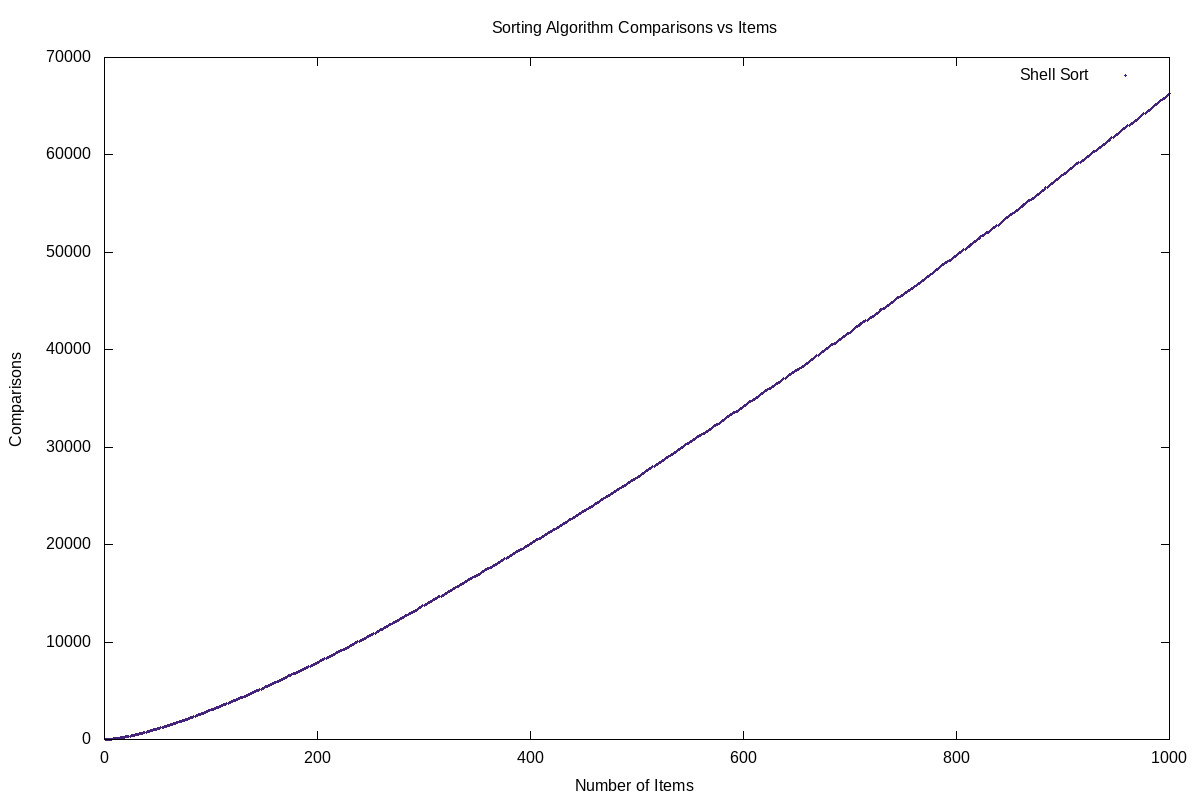
\includegraphics[width=6in]{shell}
		\centering
	\end{figure}

	\pagebreak

%%%%%%%%%%%%%%%%%%%%%%%%%%%%%%%%%%%%%%%%%%%%%%%%%%%%%%%%%%%%%%%%%%%%%%%%%%%%%%%%

	\subsection{Quicksort}

	Quicksort preformed the best by far.
	Similar to Shell Sort, Quicksort has an average case of $O(n log n)$.
	By breaking down sorting into partitions, the algorithm is able to organize the items more generally
	first, than more accurately later.
	Quicksort's worst case scenario is $O(n^2)$, but this only happens when the pivot leaves a single element on one side.
	This programs implementation of Quicksort picks the middle element as the pivot point.
	Therefore, if the middle of each partition was the largest element of that partition, the algorithm would run with the same amount of comparisons as bubble sort.
	This can be avoided by randomly picking a pivot point, however, for a general algorithm, it is not worth sacrificing efficiency in more cases for this specific inefficient case.

	A reversed array is not terrible for Quicksort.
	Similar to Shell Sort, the algorithm sorts more generally first making it pretty efficient at reversed sorted arrays.

	Although Quicksort is the fastest out of all the algorithms in the program, its efficiency constant is the biggest making it less suited for smaller arrays.
	Quicksort has to constantly push and pop to container datatype, accessing memory multiple times every iteration.
	Th
	

	Since both Quicksort implementations executed with identical swaps and comparisons,
	the graphs are identical and only the stack implementation is shown in figure \ref{stack} below.

	\begin{figure}[H]
		\caption{Quicksort (Stack)}\label{stack}
		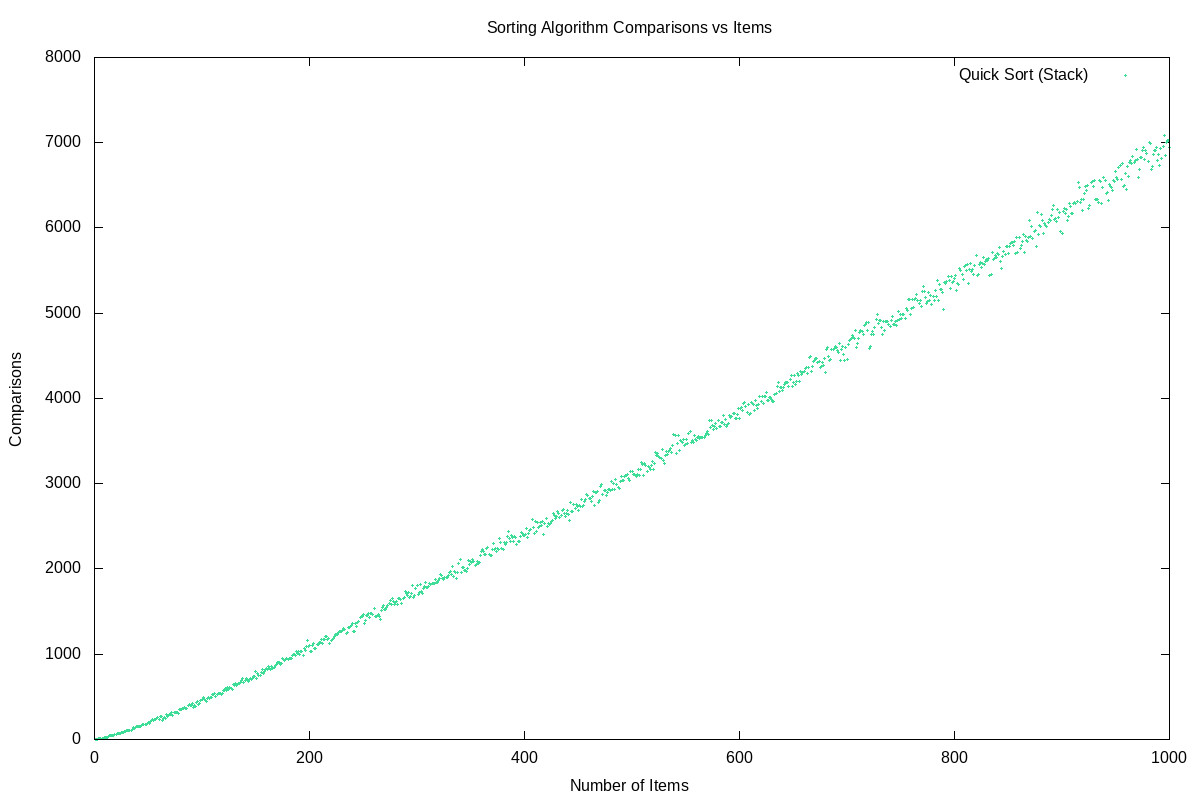
\includegraphics[width=6in]{quick_stack}
		\centering
	\end{figure}

	Although the two variants of Quicksort perform the same amount of comparisons and swaps,
	the max size of their respective containers are drastically different.
	Figure \ref{quick_size} shows how a queue makes the number of stored partition indices increase drastically.
	This increase is obviously due to the first in last out nature of a queue.
	Since a stack is first in first out, that means it sorts are partition as soon as it stores it.
	This gives the datatype a fixed size as indices are accessed depth first.
	However with a queue, more and more partitions indices are stored before they are sorted resulting in a linearly increasing size.

	\begin{figure}[H]
		\caption{Quicksort Data Structure Size Comparison}\label{quick_size}
		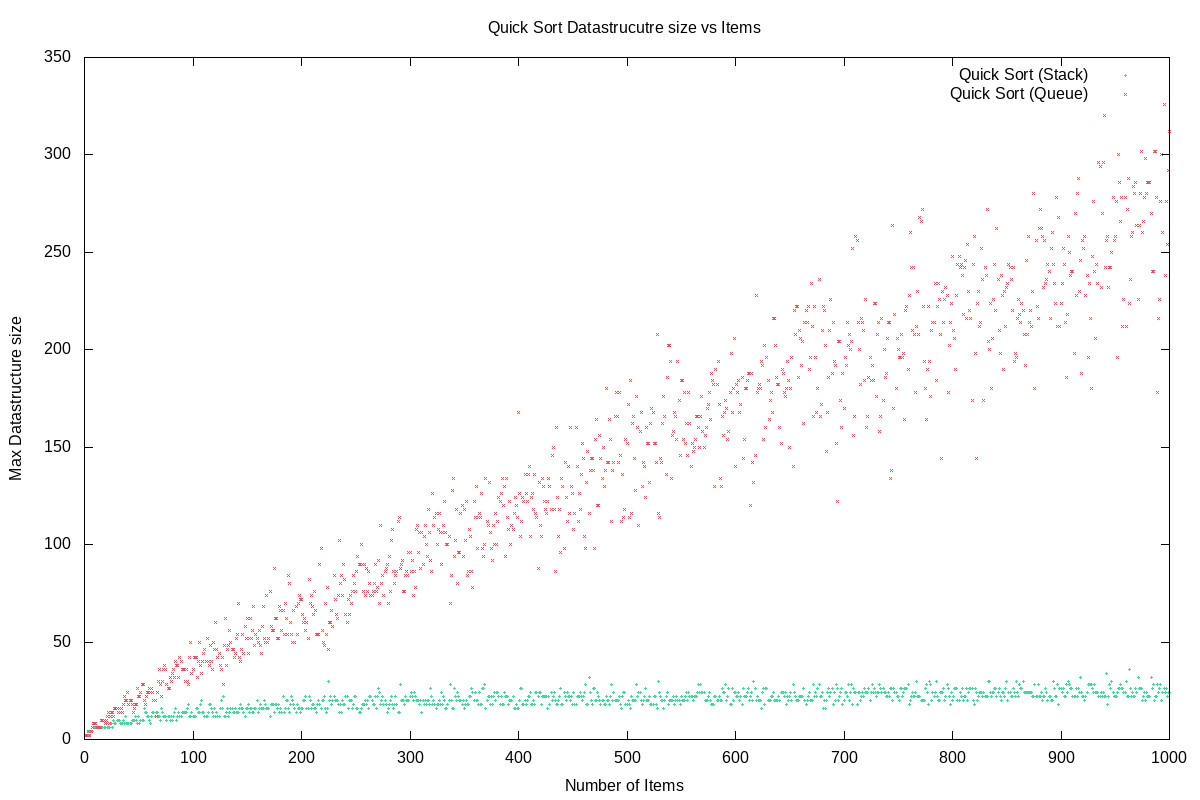
\includegraphics[width=6in]{quick_comparison_size}
		\centering
	\end{figure}

%%%%%%%%%%%%%%%%%%%%%%%%%%%%%%%%%%%%%%%%%%%%%%%%%%%%%%%%%%%%%%%%%%%%%%%%%%%%%%%%

	\subsection{Overall}

	The inefficiency of bubble sort in large arrays becomes blatantly apparent when using large numbers.
	Figure \ref{comparison} illustrates the small number of comparisons of Quicksort and Shell Sort compared to the quadratically increasing Bubble Sort.
	However, number of comparisons is not the only factor in comparing sorting algorithms.
	As previously discussed, each algorithm has a constant in addition to its big-$O$ analysis.
	When other processes are added to each loop, the execution time increases.
	Although this is a necessary evil in creating efficient algorithms for large arrays, this extra overhead slows down there are not so many elements.
	For example, figure \ref{comparison_small} seems to show that bubble sort is still slow with smaller arrays.
	However, using C's time library, the actual execution time shows Bubble Sort to be much more favorable.
	Figure \ref{time} shows that both Bubble and Shell Sort are actually faster or as fast with arrays up to 50 elements.
	
	\begin{figure}[H]
		\caption{Overall Comparison}\label{comparison}
		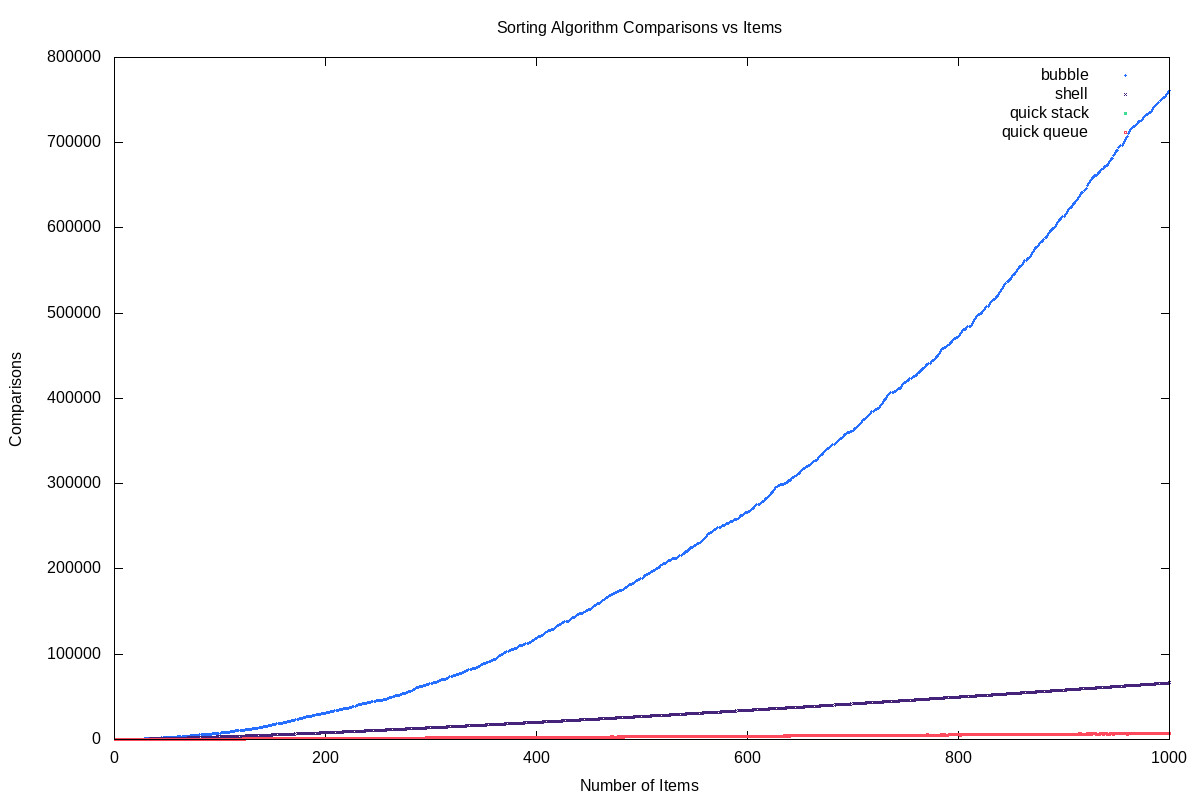
\includegraphics[width=6in]{comparison}
		\centering
	\end{figure}

	\begin{figure}[H]
		\caption{Overall Comparison With a Small Array}\label{comparison_small}
		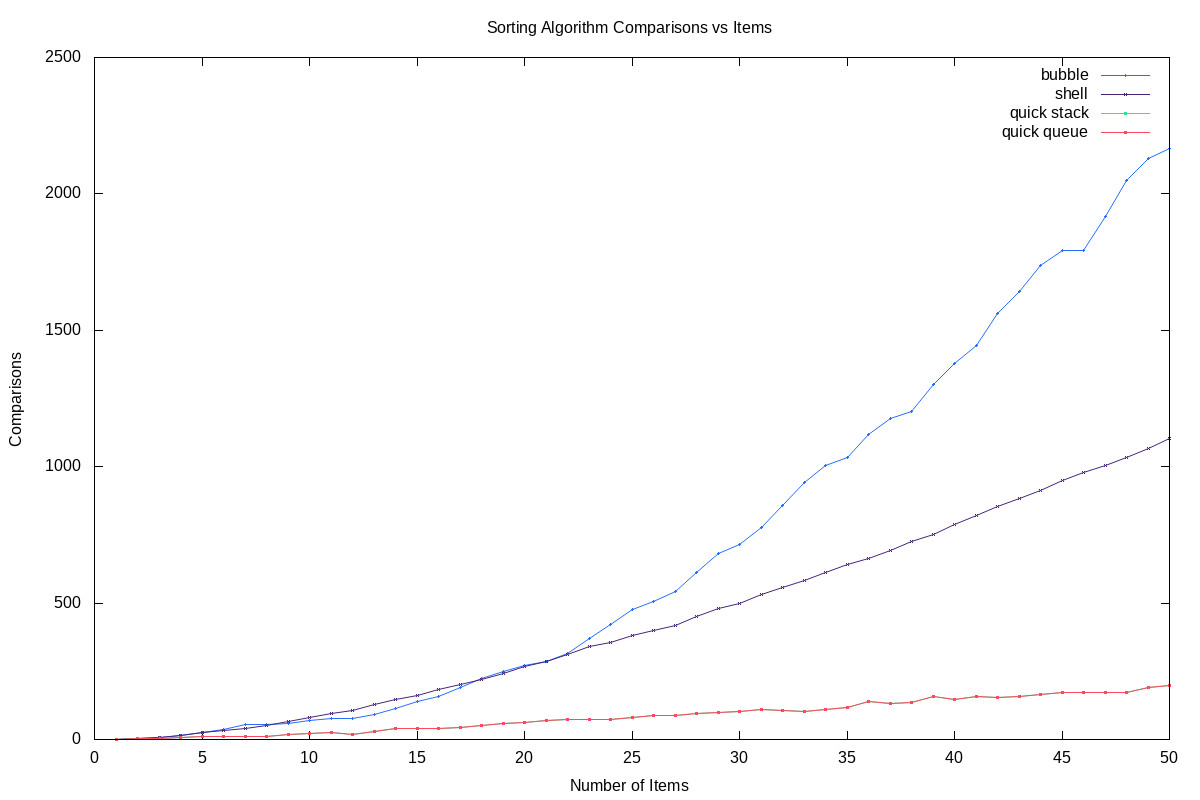
\includegraphics[width=6in]{comparison_small}
		\centering
	\end{figure}

	\begin{figure}[H]
		\caption{Overall Time With a Small Array}\label{time}
		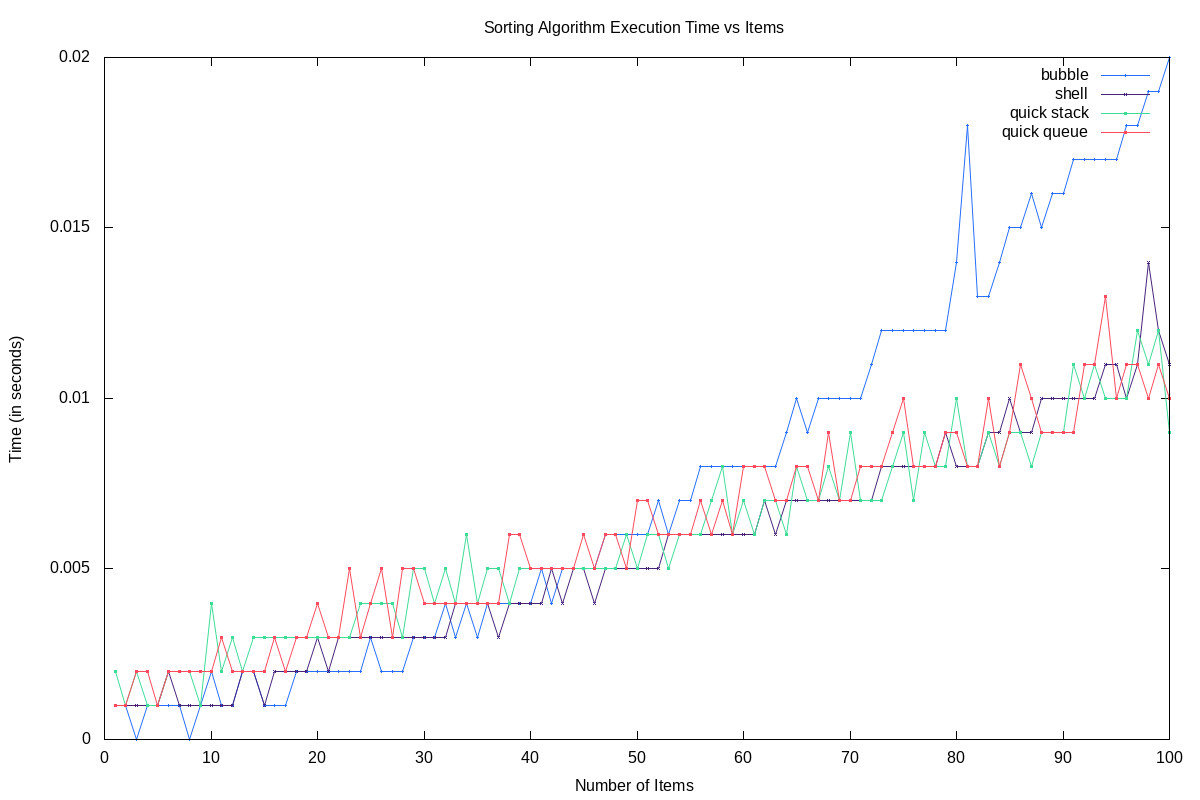
\includegraphics[width=6in]{comparison_time}
		\centering
	\end{figure}

%%%%%%%%%%%%%%%%%%%%%%%%%%%%%%%%%%%%%%%%%%%%%%%%%%%%%%%%%%%%%%%%%%%%%%%%%%%%%%%%

	\section{What I Learned}

	After this lab I learned that picking the right algorithm is crucial for accomplishing fast code.
	As shown in my experiments, "right" does not necessarily mean smallest Big-$O$ or even fastest execution time.
	It is about maximizing the performance given the constraints.

	\end{document}

